\documentclass[11pt]{article}
\usepackage[margin=0.75in]{geometry}
\usepackage{hyperref}
\usepackage{amsmath}
\usepackage{setspace}
\usepackage{booktabs}
\usepackage{graphicx}
\usepackage{float}
\usepackage[numbers]{natbib}

\hypersetup{colorlinks=true, urlcolor=blue!60!black, citecolor=blue!60!black}
\setstretch{1.0}
\setlength{\parindent}{0pt}

\title{\textbf{Prior Sensitivity in Bayesian Logistic Regression:\\
A Small-Sample Medical Study}}
\author{
    William Chen\\
    \textit{University of California, Irvine}\\
    Instructor: Prof.\ Weining Shen\\
    \textit{Stat 205P: Bayesian Data Analysis}
}
\date{}

\begin{document}
\maketitle

% -------------------------------------------------------
\begin{abstract}
In Bayesian logistic regression, the choice of prior is
inconsequential when data are plentiful but decisive when they are
scarce.
We demonstrate this using the \texttt{birthwt} dataset ($n = 189$),
comparing three priors (diffuse $\mathcal{N}(0, 100)$, weakly
informative $\mathcal{N}(0, 2.5)$, and a clinically informative prior)
across the full sample and subsamples of $n \in \{20, 40, 80, 189\}$.
At full data all three are interchangeable (AUC $\approx 0.747$; LOOIC difference $< 4$).
Under small samples they are not: at $n = 20$ the diffuse prior
collapses under complete separation
($\hat{\beta}_{\texttt{smoke1}} = 203$) while the regularizing priors
stay stable.
Crucially, how quickly a coefficient escapes prior sensitivity is
governed not by sample size but by the number of positive cases for
that predictor: smoking stabilizes by $n = 40$, whereas hypertension
(only 6.3\% of patients) remains unstable until $n \approx 80$.
For small clinical datasets the recommendation is concrete: prefer
a weakly informative prior to a diffuse one, and treat rare predictors
with particular caution, since they are the last to shed the prior's
influence.
\end{abstract}

% -------------------------------------------------------
\section{Introduction}

In Bayesian analysis the prior's influence grows as data shrink: when
samples are scarce it can substantially shape, and even distort, the
posterior---a concern that is especially acute in clinical research.
This report presents a prior sensitivity analysis of Bayesian logistic
regression using the \texttt{birthwt} dataset ($n = 189$), comparing
three priors (diffuse $\mathcal{N}(0,100)$, weakly informative
$\mathcal{N}(0,2.5)$, and a clinically informative prior) refitted
across $n \in \{20, 40, 80, 189\}$.
We find that sensitivity is governed not by sample size alone but by
predictor rarity, with direct implications for clinical datasets where
the most important risk factors are often uncommon.

% -------------------------------------------------------
\section{Data}

\subsection{Dataset Overview}

The \texttt{birthwt} dataset ($n = 189$) was collected at Baystate
Medical Center, Springfield, MA (1986).
The binary outcome is low birth weight ($< 2.5$ kg), with 130 normal
and 59 low birth weight cases (31.2\% positive rate).
All analyses use \texttt{stan\_glm} (\texttt{rstanarm}), fit with
4 chains $\times$ 1000 iterations.

\subsection{Predictors}

Predictors include maternal age, pre-pregnancy weight, race,
smoking status, prior preterm labor, hypertension history (\texttt{ht}),
uterine irritability (\texttt{ui}), and first-trimester physician visits.
Among the binary predictors, positive cases are sparse and uneven:
74/189 for smoking, 28 for uterine irritability, and only 12 for
hypertension---a spread that becomes consequential under small samples.

% -------------------------------------------------------
\section{Methods}

\subsection{Prior Specification}

Three prior configurations were evaluated:

\begin{center}
\begin{tabular}{lll}
\toprule
Model & Coefficients & Intercept \\
\midrule
Diffuse      & $\mathcal{N}(0,\,100)$
             & $\mathcal{N}(0,\,100)$ \\
Weak         & $\mathcal{N}(0,\,2.5)$
             & $\mathcal{N}(0,\,10)$  \\
Informative  & \texttt{smoke}, \texttt{ht}: $\mathcal{N}(1,\,0.5)$;
               others $\mathcal{N}(0,\,1)$
             & $\mathcal{N}(0,\,5)$   \\
\bottomrule
\end{tabular}
\end{center}

The informative prior encodes clinical knowledge: $\mathcal{N}(1, 0.5)$
for \texttt{smoke} and \texttt{ht} corresponds to OR $\approx 2.7$
($\pm 2$ SD: OR $\in [1.4, 7.4]$), consistent with published estimates
\cite{Simpson1957,Shah2000}. All other predictors use $\mathcal{N}(0,1)$.

\subsection{Analyses}

We conduct three analyses: (1) full-data prior comparison via
posterior coefficients, LOO-CV, and AUC; (2) a subsampling experiment
refitting all models at $n \in \{20, 40, 80, 189\}$ to track
convergence across sample sizes, including a 100-draw repeated
subsampling robustness check; and (3) predictive performance assessed
via LOOIC and Pareto $\hat{k}$ diagnostics.
Convergence was verified via $\hat{R} \leq 1.002$ and trace plots.

% -------------------------------------------------------
\section{Results}

\subsection{Full Data ($n = 189$): Priors Have Little Effect}

At $n = 189$, all three models produce nearly identical posterior
estimates and converge well.
Table~\ref{tab:coef} reports posterior means for the two clinically
relevant predictors, and Figure~\ref{fig:coef} shows the full
coefficient comparison across all predictors.

\begin{table}[H]
\centering
\begin{tabular}{lcccccc}
\toprule
 & \multicolumn{2}{c}{Diffuse} & \multicolumn{2}{c}{Weak} & \multicolumn{2}{c}{Informative} \\
\cmidrule(lr){2-3}\cmidrule(lr){4-5}\cmidrule(lr){6-7}
Variable & Mean & 95\% CI & Mean & 95\% CI & Mean & 95\% CI \\
\midrule
\texttt{smoke1} & 0.983 & [0.21, 1.83] & 0.933 & [0.13, 1.74] & 0.915 & [0.31, 1.52] \\
\texttt{ht1}    & 1.994 & [0.63, 3.50] & 1.827 & [0.49, 3.30] & 1.311 & [0.51, 2.13] \\
\bottomrule
\end{tabular}
\caption{Posterior means and 95\% credible intervals (log-odds) for the two clinically targeted
predictors at $n = 189$.}
\label{tab:coef}
\end{table}

\begin{figure}[htbp]
    \centering
    \begin{minipage}{0.44\textwidth}
        \centering
        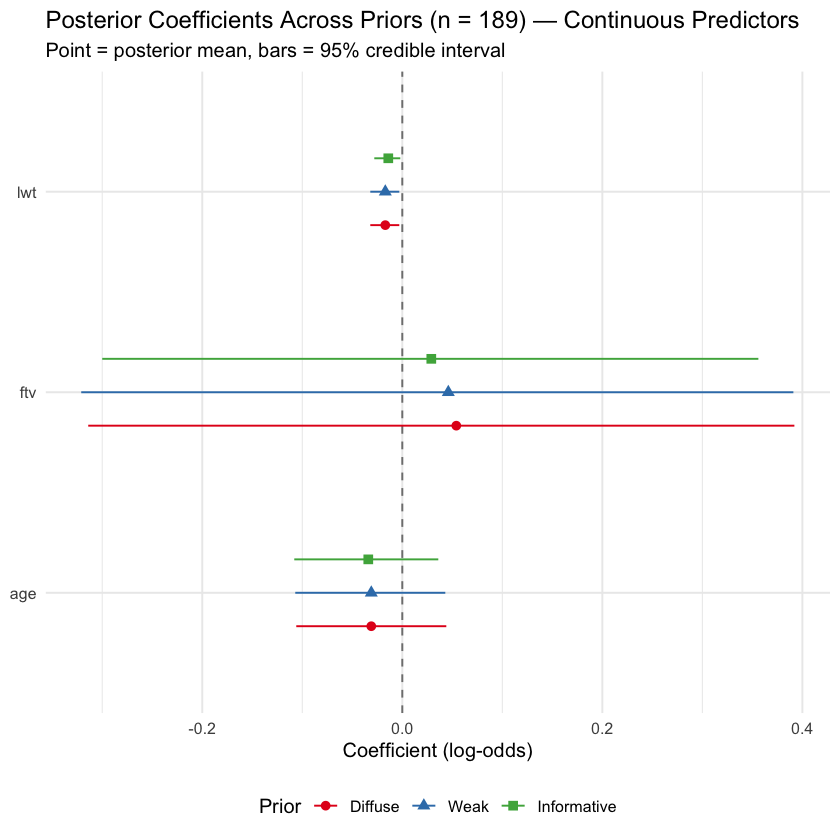
\includegraphics[width=\textwidth]{../figures/coef_continuous.png}
    \end{minipage}
    \hfill
    \begin{minipage}{0.44\textwidth}
        \centering
        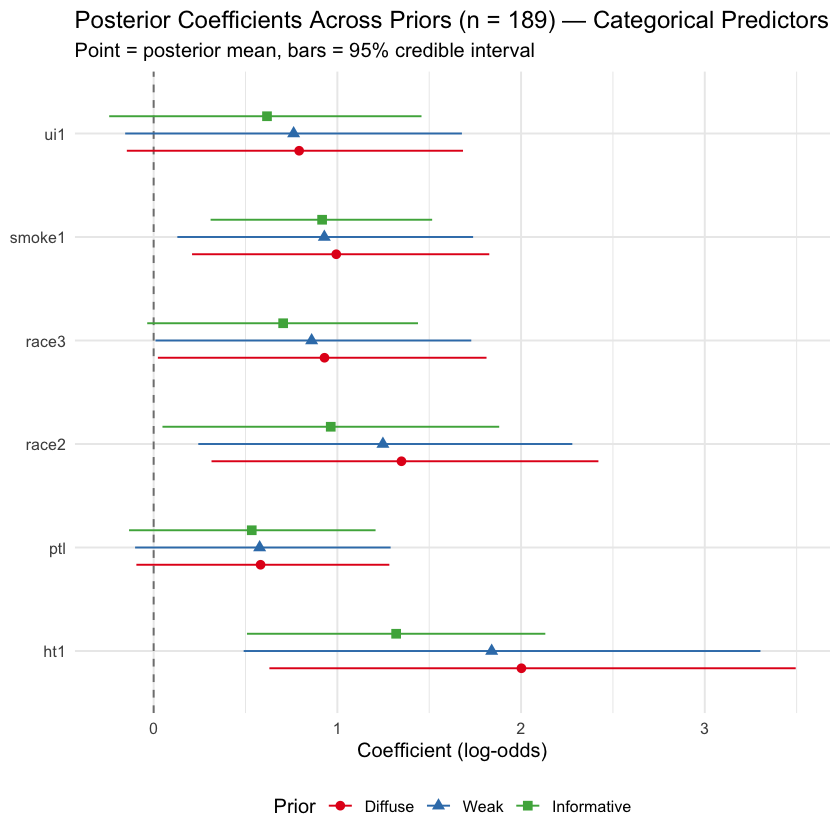
\includegraphics[width=\textwidth]{../figures/coef_binary.png}
    \end{minipage}
    \caption{Posterior coefficients across priors at $n = 189$.
    Left: continuous predictors. Right: categorical/binary predictors.
    Points = posterior mean; bars = 95\% credible interval.}
    \label{fig:coef}
\end{figure}

The informative prior modestly shrinks \texttt{ht1} (from 1.994 to
1.311), but this difference is small in practical terms.
Table~\ref{tab:loo_auc} reports LOO and AUC for all three models;
the differences are negligible, confirming that prior choice has
little practical effect at $n = 189$.

\begin{table}[H]
\centering
\begin{tabular}{lcc}
\toprule
Model & LOOIC & AUC \\
\midrule
Diffuse     & 223.85 & 0.746 \\
Weak        & 223.32 & 0.747 \\
Informative & 220.43 & 0.748 \\
\bottomrule
\end{tabular}
\caption{LOO model comparison and AUC at full data ($n = 189$).
Lower LOOIC indicates better fit.}
\label{tab:loo_auc}
\end{table}


\subsection{Subsampling: Prior Sensitivity at Small $n$}

To examine how prior influence changes with sample size, we refit all
three models at $n \in \{20, 40, 80, 189\}$.
We focus on \texttt{smoke1} and \texttt{ht1}, the two predictors
for which the informative prior encodes directional knowledge,
as these show the largest divergence across priors at small $n$
(Figure~\ref{fig:convergence}).

\begin{figure}[htbp]
    \centering
    \begin{minipage}{0.42\textwidth}
        \centering
        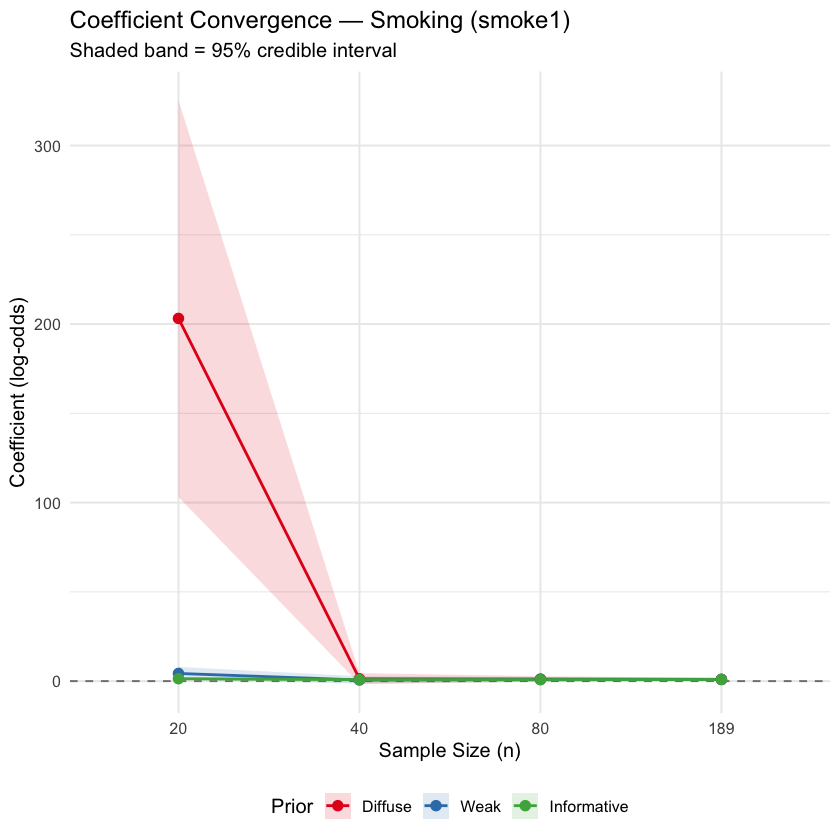
\includegraphics[width=\textwidth]{../figures/smoke_convergence.png}
    \end{minipage}
    \hfill
    \begin{minipage}{0.42\textwidth}
        \centering
        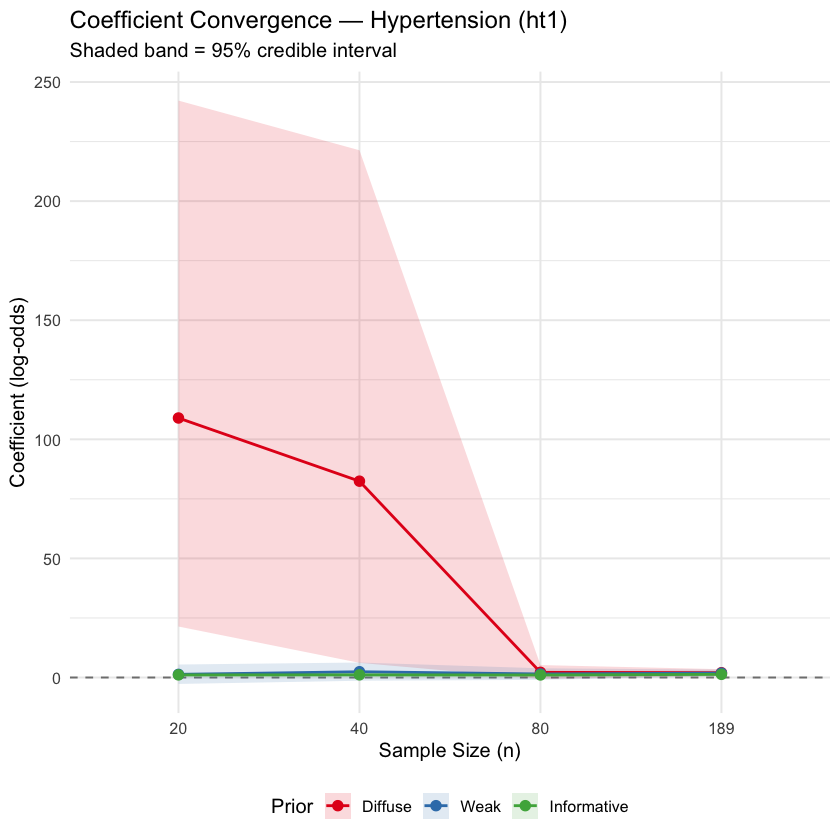
\includegraphics[width=\textwidth]{../figures/ht_convergence.png}
    \end{minipage}
    \caption{Posterior mean convergence. Left: \texttt{smoke1}.
    Right: \texttt{ht1}. Shaded bands = 95\% credible intervals.}
    \label{fig:convergence}
\end{figure}

Under the diffuse prior, complete separation produces implausible
estimates at $n = 20$ ($\hat{\beta}_{\texttt{smoke1}} = 203$,
$\hat{\beta}_{\texttt{ht1}} = 109$).
\texttt{smoke1} recovers by $n = 40$, but \texttt{ht1} remains
unstable ($\hat{\beta} = 82.4$): hypertension affects only 12 of
189 patients (6.3\%), so small subsamples rarely contain enough
\texttt{ht} = 1 cases to resolve separation.
By $n = 80$, all models stabilize.
The weak and informative priors remain in clinically plausible ranges
throughout.
(These coefficient values are from a single representative draw with
\texttt{set.seed(42)}; the robustness check below confirms they are
typical rather than exceptional.)

\subsubsection*{Robustness Check: Repeated Subsampling}

To confirm that these thresholds are not artefacts of a single random
draw, we repeated the subsampling 100 times per $n$ with independent
seeds and recorded the proportion of runs in which the diffuse prior
produced $|\hat{\beta}| > 10$ (Figure~\ref{fig:blowup}).
At $n = 20$, \texttt{ht1} explodes in 31.1\% of draws (and is
undefined---no \texttt{ht}$= 1$ case sampled---in a further 26\%).
\texttt{smoke1} and \texttt{ui1} largely stabilize by $n = 40$
(explosion rates $\leq 3\%$), while \texttt{ht1} persists at 17.6\%
at $n = 40$ and reaches zero only at $n = 80$.
The single-draw results above are therefore representative, not
coincidental.

\begin{figure}[htbp]
    \centering
    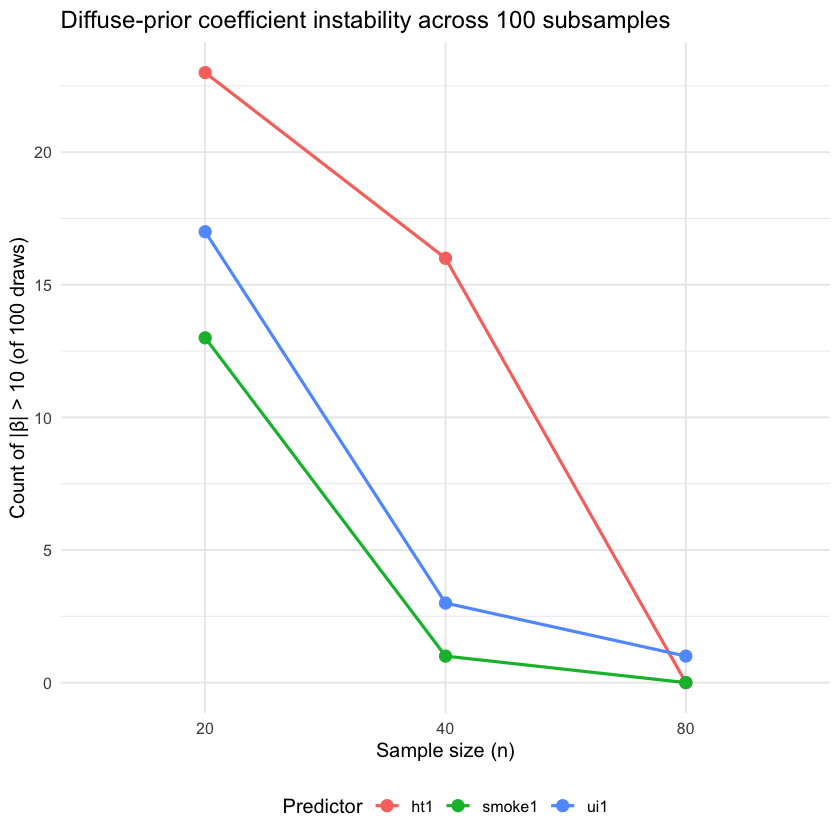
\includegraphics[width=0.42\textwidth]{../figures/fig_coef_blowup.png}
    \caption{Subsamples (out of 100) where diffuse prior yields
    $|\hat{\beta}| > 10$. \texttt{ht1} is last to stabilize.}
    \label{fig:blowup}
\end{figure}

\subsection{Predictive Performance}

In-sample AUC is unreliable under separation; we use LOOIC and
Pareto $\hat{k}$ diagnostics instead (Table~\ref{tab:loo_sub}).
At $n = 20$ the diffuse prior's AUC $= 1.0$ reflects overfitting,
confirmed by 20 problematic $\hat{k}$ values and a spuriously low
LOOIC of 8.3. The informative prior remains reliable throughout
(1 problematic observation at $n = 20$) and achieves the lowest
LOOIC at every sample size, including full data
(Informative $= 220.4$, Weak $= 223.3$, Diffuse $= 223.8$).

\begin{table}[H]
\centering
\begin{tabular}{llccc}
\toprule
$n$ & Model & AUC & LOOIC & $\hat{k}>0.7$ \\
\midrule
20 & Diffuse     & 1.000 &  8.3 & 20 \\
20 & Weak        & 0.952 & 28.1 &  5 \\
20 & Informative & 0.905 & 27.1 &  1 \\
\midrule
40 & Diffuse     & 0.808 & 65.3 &  4 \\
40 & Weak        & 0.799 & 61.1 &  0 \\
40 & Informative & 0.750 & 56.3 &  1 \\
\midrule
80 & Diffuse     & 0.789 & 105.9 & 0 \\
80 & Weak        & 0.785 & 102.4 & 1 \\
80 & Informative & 0.777 &  98.2 & 0 \\
\bottomrule
\end{tabular}
\caption{In-sample AUC, LOOIC, and Pareto $\hat{k}>0.7$ count by
sample size and prior. At $n=20$ the diffuse prior's LOOIC and AUC
are both unreliable.}
\label{tab:loo_sub}
\end{table}

% -------------------------------------------------------
\section{Discussion}

\paragraph{Two distinct mechanisms.}
Prior sensitivity at small $n$ operates through two channels.
The first is \emph{separation stabilization}: when no positive cases
are sampled, the likelihood is uninformative and a diffuse prior lets
coefficients diverge---a problem frequentist MLE shares.
A weakly informative prior acts as a regularizer, keeping estimates
in a plausible range until more data arrive.
The second is \emph{gentle posterior shrinkage}: even without
separation, an informative prior pulls estimates toward clinical
expectations, as seen in \texttt{ht1} shifting from 1.994 (diffuse)
to 1.311 (informative) at $n = 189$. These are related but distinct,
and both are present in this analysis.

\paragraph{Limitations.}
Results derive from a single dataset; generalizability requires
validation. At very small $n$, LOO is unreliable
(Pareto $\hat{k} > 0.7$); $k$-fold cross-validation is more
appropriate in such settings.

% -------------------------------------------------------
\section{Conclusion}

Prior choice matters most when data are scarcest. At $n = 20$ a
diffuse prior produces unstable, uninterpretable posteriors while a
weakly informative prior restores stability; by $n = 189$ the
differences are negligible. Crucially, the threshold is not uniform:
at $n = 20$ no predictor is reliable; by $n = 40$, two of three
have stabilized---only hypertension remains, and it persists until
$n = 80$, confirmed across 100 repeated draws. The governing factor is not
sample size but the number of positive cases: smoking (74) and uterine
irritability (28) recover together, while hypertension (12) is last.

For small clinical datasets the takeaway is direct: make a weakly
informative prior the default, and treat rare predictors with
particular caution---they are the last to shed the prior's influence.

% -------------------------------------------------------
\begin{thebibliography}{9}

\bibitem{Simpson1957}
Simpson, W.J. (1957).
A preliminary report on cigarette smoking and the incidence of
prematurity.
\textit{American Journal of Obstetrics and Gynecology}, 73(4), 807--815.

\bibitem{Shah2000}
Shah, N.R., \& Bracken, M.B. (2000).
A systematic review and meta-analysis of prospective studies on the
association between maternal cigarette smoking and preterm delivery.
\textit{American Journal of Obstetrics and Gynecology}, 182(2), 465--472.

\end{thebibliography}

\end{document}